\documentclass{report}
\usepackage[utf8]{inputenc}
\usepackage[spanish]{babel}
\usepackage[margin=2cm]{geometry}
\usepackage{graphicx}
\usepackage{float}
\usepackage{titlesec}
\usepackage{caption}
\usepackage{listings}
\usepackage{xcolor}
\usepackage{array}
\usepackage{booktabs}
\usepackage{tabularx}
\usepackage{multirow}
\usepackage{amsmath}
\usepackage{hyperref}

\definecolor{codegreen}{rgb}{0,0.6,0}
\definecolor{codegray}{rgb}{0.5,0.5,0.5}
\definecolor{codepurple}{rgb}{0.58,0,0.82}
\definecolor{backcolor}{rgb}{0.95,0.95,0.95}


\lstset{
    basicstyle=\ttfamily,
    inputencoding=utf8,
    extendedchars=true,
    literate=%
    {á}{{\'a}}1
    {é}{{\'e}}1
    {í}{{\'i}}1
    {ó}{{\'o}}1
    {ú}{{\'u}}1
    {ñ}{{\~n}}1
    {Á}{{\'A}}1
    {É}{{\'E}}1
    {Í}{{\'I}}1
    {Ó}{{\'O}}1
    {Ú}{{\'U}}1
    {Ñ}{{\~N}}1
}


\lstdefinestyle{mystyle}{
    backgroundcolor=\color{backcolor},
    commentstyle=\color{codegreen},
    keywordstyle=\color{red},
    numberstyle=\tiny\color{codegray},
    stringstyle=\color{codepurple},
    basicstyle=\ttfamily\footnotesize,
    breakatwhitespace=false,
    breaklines=true,
    captionpos=b,
    keepspaces=true,
    numbers=left,
    showspaces=false,
    showstringspaces=false,
    showtabs=false,
    tabsize=2  
}

\titleformat{\section}
{\huge\bfseries}{\thesection.}{1em}{}
\titleformat{\subsection}
{\large\bfseries}{\thesubsection}{1em}{}

\renewcommand\thesection{\arabic{section}}

\title{\Huge{\textbf{Práctica: Clasificación de sonidos.}}\\
\Large{\textbf{Reconocimiento de Voz}}}
\author{Escamilla Resendiz Aldo}

\graphicspath{{imagenes/}}

\begin{document}
    \maketitle
    \tableofcontents
    \newpage
    \section{Introducción}

    En esta práctica, se realizó el procesamiento de archivos de audio con el objetivo de segmentarlos en intervalos de 100 milisegundos y extraer características clave de cada segmento. Entre las características analizadas se encuentran la \textbf{amplitud media}, el \textbf{valor RMS} (\textit{Root Mean Square}) y la \textbf{tasa de cruces por cero}. Estas métricas permiten obtener una representación detallada del comportamiento de la señal de audio a lo largo del tiempo.

    Para la clasificación de los segmentos de audio, se utilizó un \textbf{árbol de decisión}, un algoritmo de aprendizaje supervisado que permite etiquetar cada segmento en función de su contenido sonoro. En este caso, las etiquetas asignadas fueron \textbf{S}, \textbf{U} y \textbf{V}, las cuales representan diferentes categorías dentro del audio procesado. El modelo de clasificación fue entrenado con estos datos y posteriormente evaluado para medir su precisión en la predicción de nuevas muestras.

    El modelo generado facilita la identificación de patrones en los segmentos de audio y permite visualizar cómo las características extraídas influyen en la clasificación. Este procedimiento es aplicable en diversas áreas, como el reconocimiento de voz, la detección de eventos acústicos y la categorización automática de sonidos.
    \section{Desarrollo}

\subsection{Herramientas utilizadas}
Para la implementación de la práctica, se emplearon las siguientes herramientas:

\begin{itemize}
    \item \textbf{Python}: Lenguaje de programación principal para la manipulación y análisis de los datos de audio.
    \item \textbf{Librosa}: Biblioteca especializada en procesamiento de señales de audio, utilizada para cargar archivos, calcular espectrogramas y extraer características acústicas.
    \item \textbf{Matplotlib}: Biblioteca de visualización que permitió graficar la forma de onda, espectrogramas y segmentaciones temporales.
    \item \textbf{Soundfile}: Utilizada para la lectura y escritura de archivos de audio en formato WAV.
\end{itemize}

\subsection{Metodología de desarrollo}
La metodología implementada se dividió en varias etapas clave:

\begin{enumerate}
    \item \textbf{Obtención de datos}: Se grabaron frases específicas en formato WAV, asegurando calidad de audio adecuada y frecuencia de muestreo constante.
    \item \textbf{Procesamiento de datos}: 
    \begin{itemize}
        \item Carga del audio con \texttt{Librosa}.
        \item Visualización de la forma de onda para identificar la estructura temporal.
        \item Segmentación del audio en bloques de 100 ms para su posterior clasificación.
    \end{itemize}
    \item \textbf{Implementación de la metodología}:
    \begin{itemize}
        \item Transformada rápida de Fourier (STFT) para obtener espectrogramas de banda ancha y estrecha.
        \item Conversión a escala logarítmica para visualizar mejor la energía de las frecuencias.
        \item Análisis de los patrones acústicos en los espectrogramas para correlacionar con eventos fonéticos específicos.
    \end{itemize}
    
\end{enumerate}

\newpage
\subsection{Código en Python}
\lstinputlisting[language=Python, style=mystyle]{p1.py}
\newpage
\section{Resultados gráficos de los audios}
A continuación, se presentan las representaciones para cinco archivos de audio:

\subsection{Audio 1 - La casa es grande.}
\begin{itemize}
    \item \textbf{Dominio del tiempo con segmentación de 100 ms y etiquetas (S, U, V)}
    \begin{figure}[h]
        \centering
        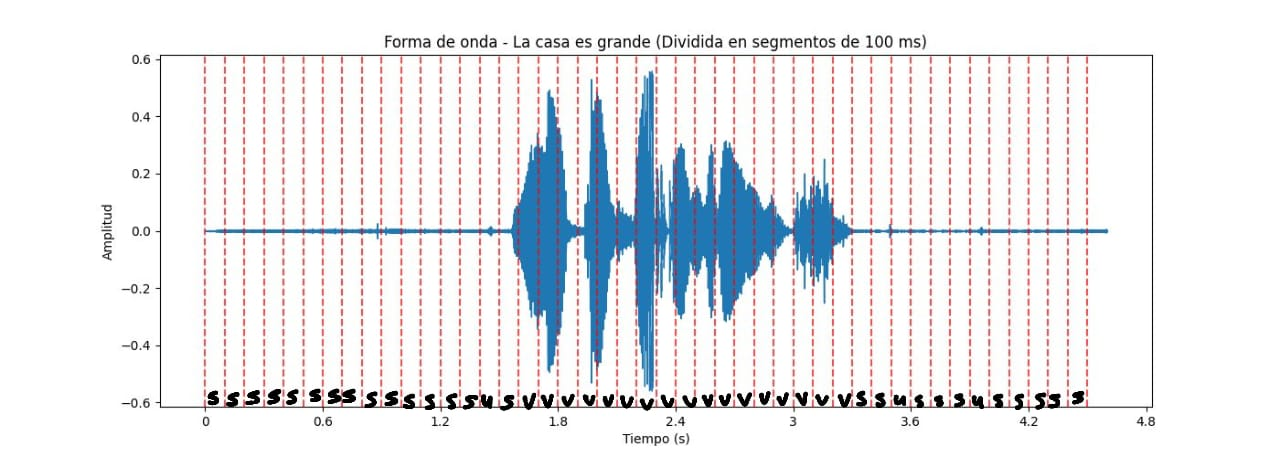
\includegraphics[width=\linewidth]{/audio1/a1.jpeg}
        \caption{Forma de onda del audio: La casa es grande, con segmentación de 100 ms}
        \label{fig:forma_onda_audio1div}
    \end{figure}
    \item \textbf{Forma de onda de la señal de voz completa}
    \begin{figure}[h]
        \centering
        \includegraphics[width=\linewidth]{/audio1/Figure_1.png}
        \caption{Forma de onda del audio: La casa es grande, con segmentación de 100 ms}
        \label{fig:forma de onda_audio1}
    \end{figure}
    \newpage
    \item \textbf{Espectrograma de banda ancha}
    \begin{figure}[h]
        \centering
        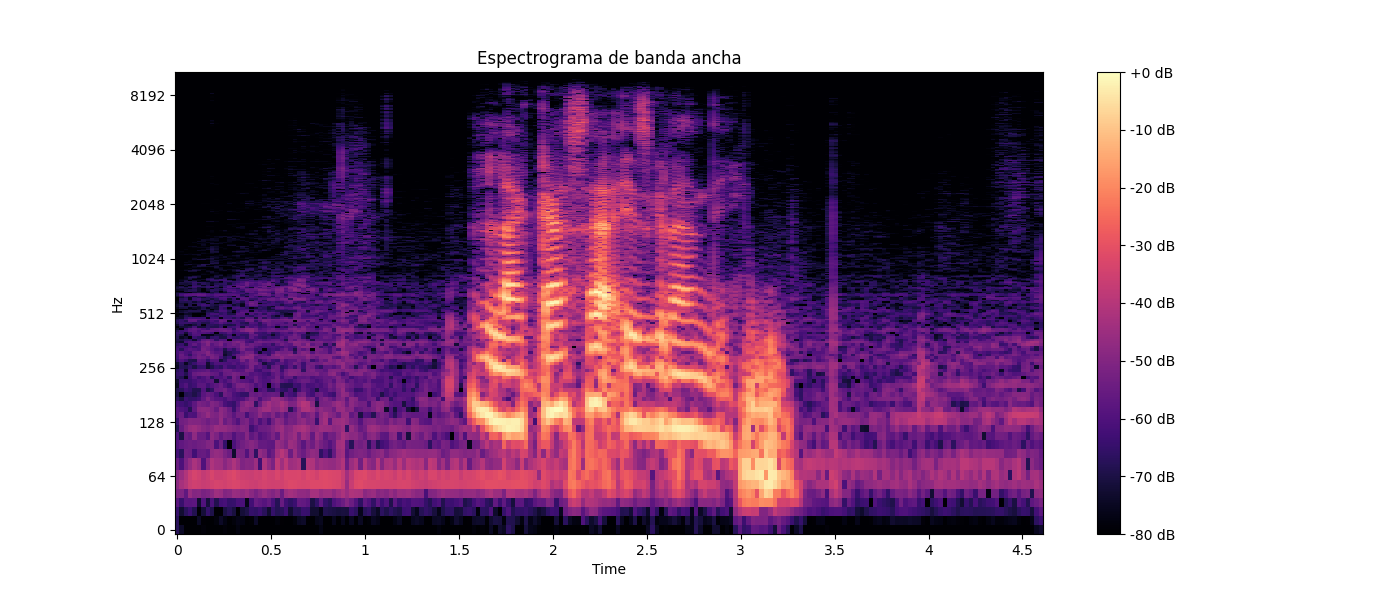
\includegraphics[width=\linewidth]{/audio1/espectogramaancha.png}
        \caption{Espectrograma de banda ancha del audio: La casa es grande}
        \label{fig:espectograma de banda ancha audio1}
    \end{figure}
    \item \textbf{Espectrograma de banda ancha}
    \begin{figure}[h]
        \centering
        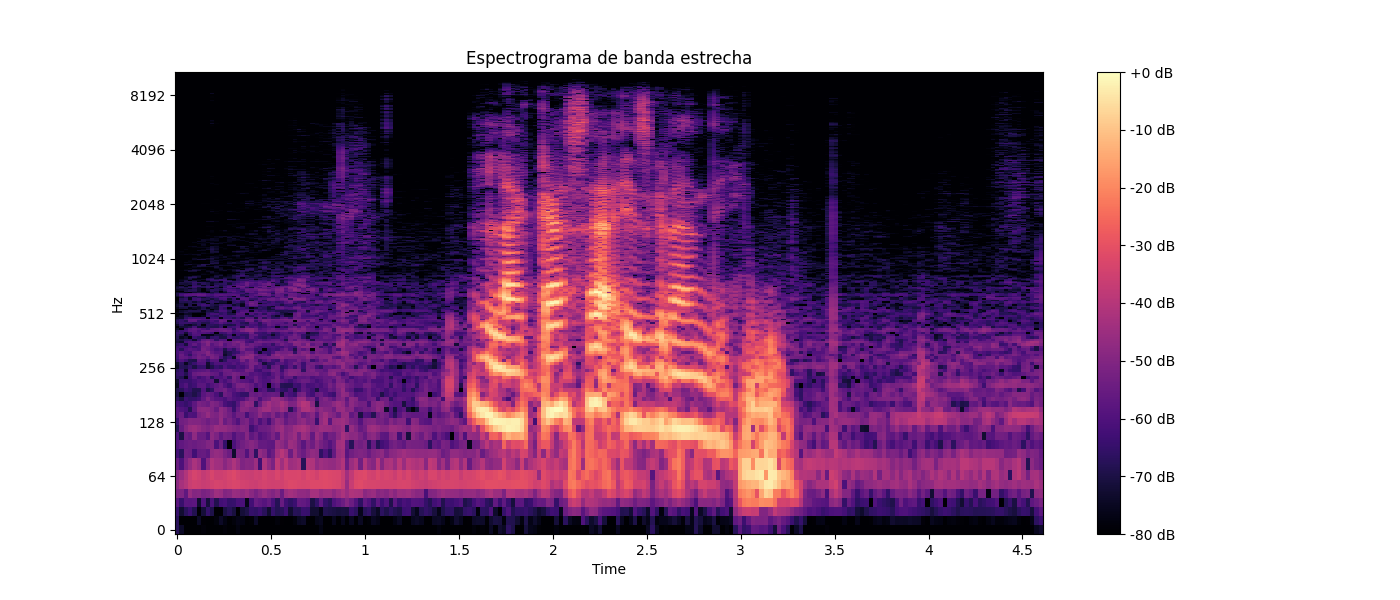
\includegraphics[width=\linewidth]{/audio1/espectogramaestreca.png}
        \caption{Espectrograma de banda estrecha del audio: La casa es grande}
        \label{fig:espectograma de banda estrecha audio1}
    \end{figure}
\end{itemize}
\newpage
\subsection{Audio 2 - Mi perro se salió de casa.}
\begin{itemize}
    \item \textbf{Dominio del tiempo con segmentación de 100 ms y etiquetas (S, U, V)}
    \begin{figure}[h]
        \centering
        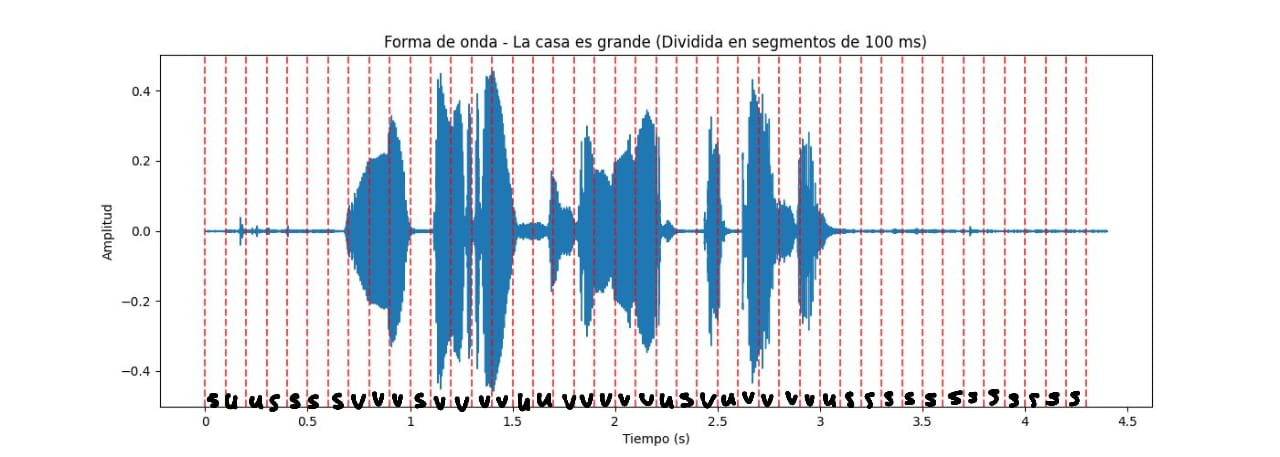
\includegraphics[width=\linewidth]{/audio2/a2.jpeg}
        \caption{Forma de onda del audio: Mi perro se salió de casa}
        \label{fig:forma_onda_audio2div}
    \end{figure}
    \item \textbf{Forma de onda de la señal de voz completa}
    \begin{figure}[h]
        \centering
        \includegraphics[width=\linewidth]{/audio2/Figure_1.png}
        \caption{Forma de onda del audio: Mi perro se salió de casa, con segmentación de 100 ms}
        \label{fig:forma_onda_audio1}
    \end{figure}
    \newpage
    \item \textbf{Espectrograma de banda ancha}
    \begin{figure}[h]
        \centering
        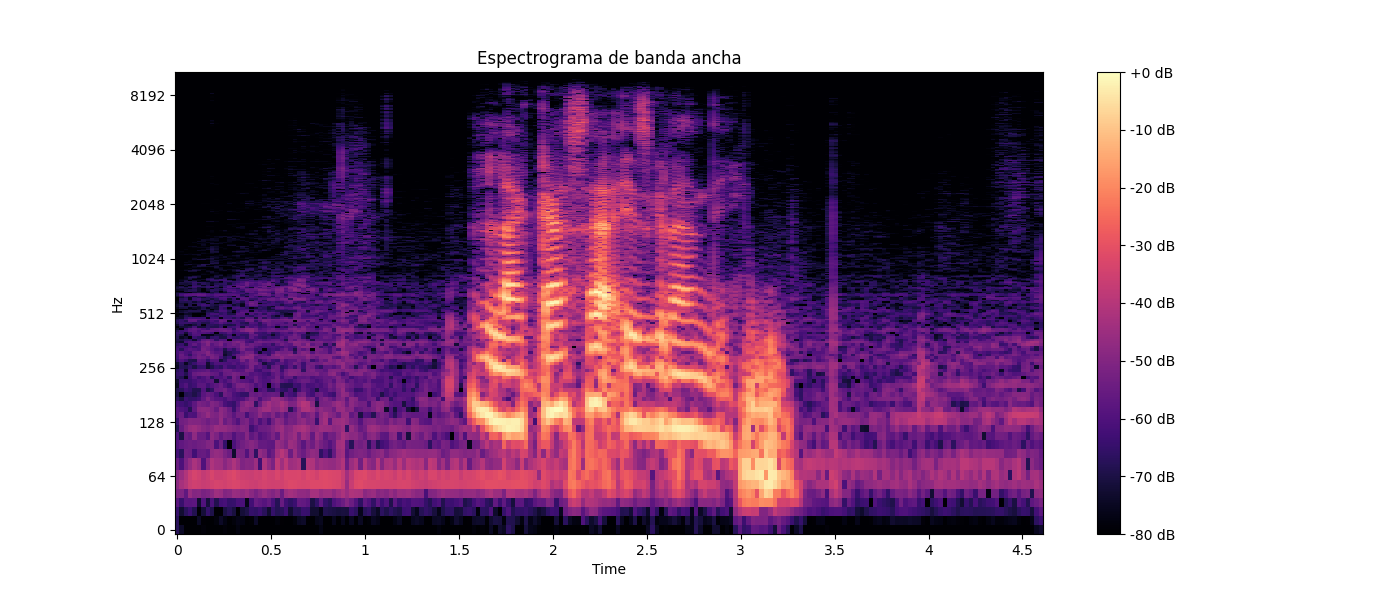
\includegraphics[width=\linewidth]{/audio1/espectogramaancha.png}
        \caption{Espectrograma de banda ancha del audio: Mi perro se salió de casa}
        \label{fig:espectograma banda ancha audio1}
    \end{figure}
    \item \textbf{Espectrograma de banda estrecha}
    \begin{figure}[h]
        \centering
        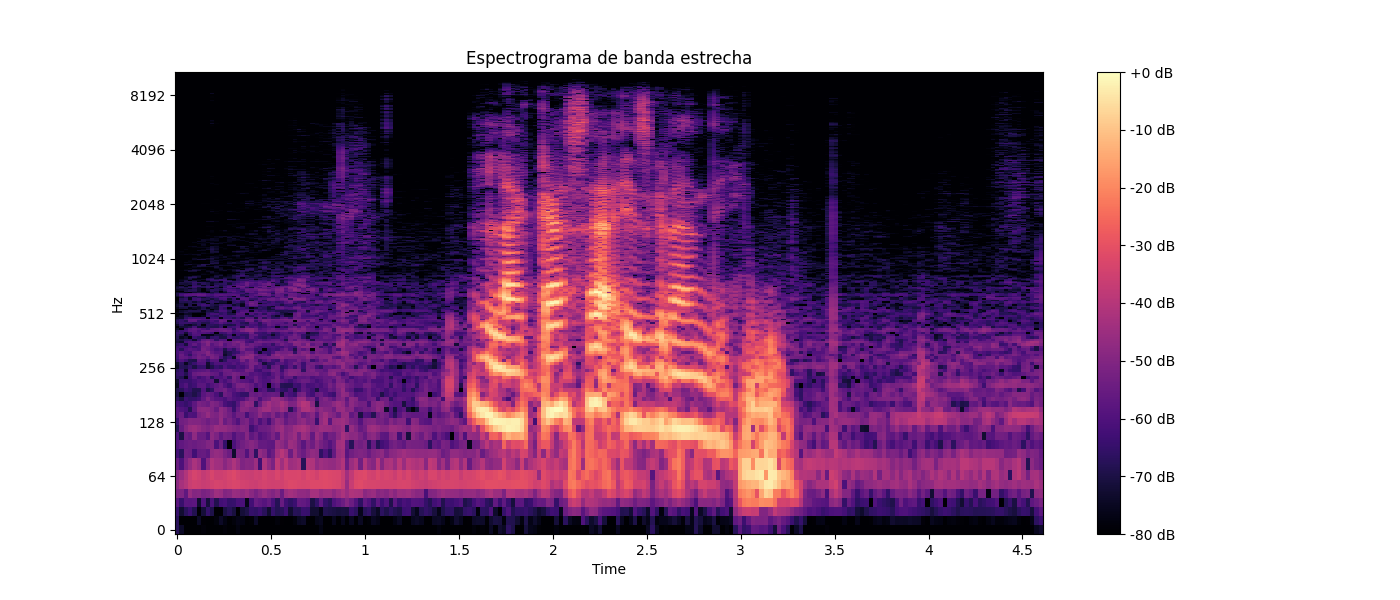
\includegraphics[width=\linewidth]{/audio1/espectogramaestreca.png}
        \caption{Espectrograma de banda estrecha del audio: Mi perro se salió de casa}
        \label{fig:espectograma banda estrecha audio1}
    \end{figure}
\end{itemize}
\newpage
\subsection{Audio 3 - Casa es a lo que llamo hogar.}
\begin{itemize}
    \item \textbf{Dominio del tiempo con segmentación de 100 ms y etiquetas (S, U, V)}
    \begin{figure}[h]
        \centering
        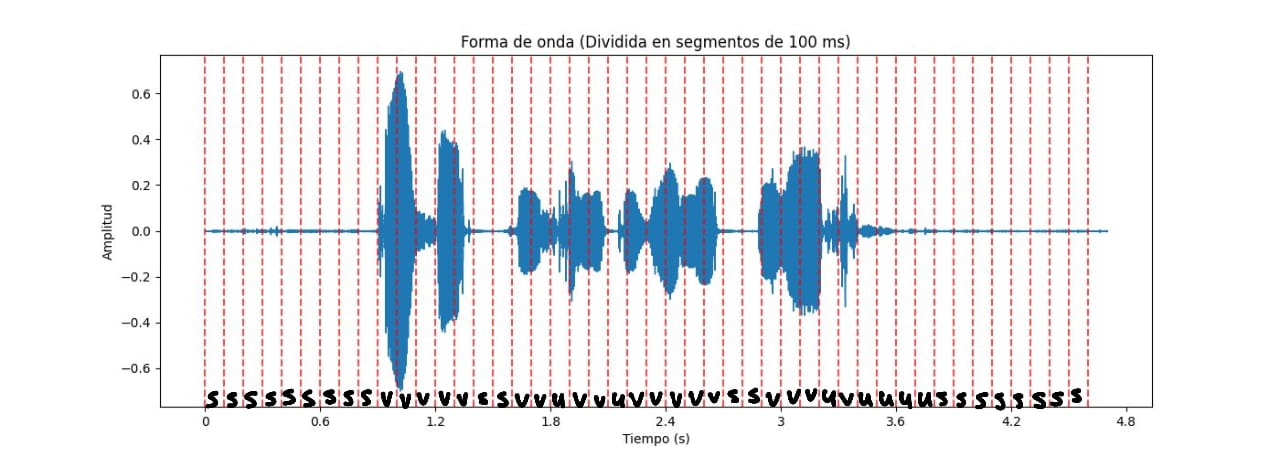
\includegraphics[width=\linewidth]{/audio3/a3.jpeg}
        \caption{Forma de onda del audio: Casa es a lo que llamo hogar.}
        \label{fig:forma_onda_audio3div}
    \end{figure}
    \item \textbf{Forma de onda de la señal de voz completa}
    \begin{figure}[h]
        \centering
        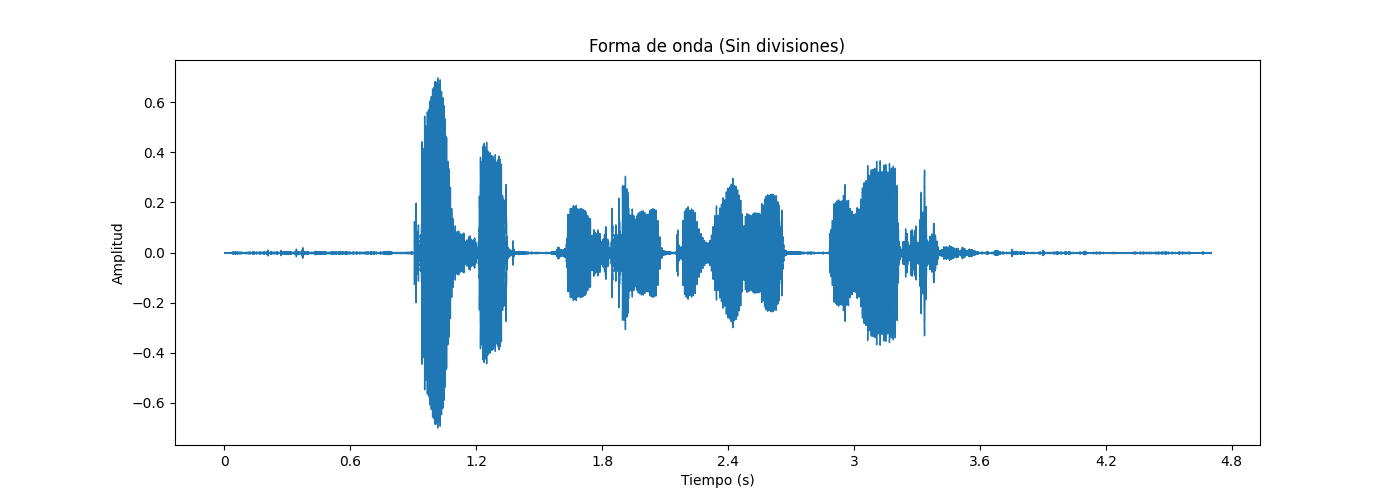
\includegraphics[width=\linewidth]{/audio3/Figure_1a3.png}
        \caption{Forma de onda del audio: Casa es a lo que llamo hogar., con segmentación de 100 ms}
        \label{fig:forma de onda_audio3}
    \end{figure}
    \newpage
    \item \textbf{Espectrograma de banda ancha}
    \begin{figure}[h]
        \centering
        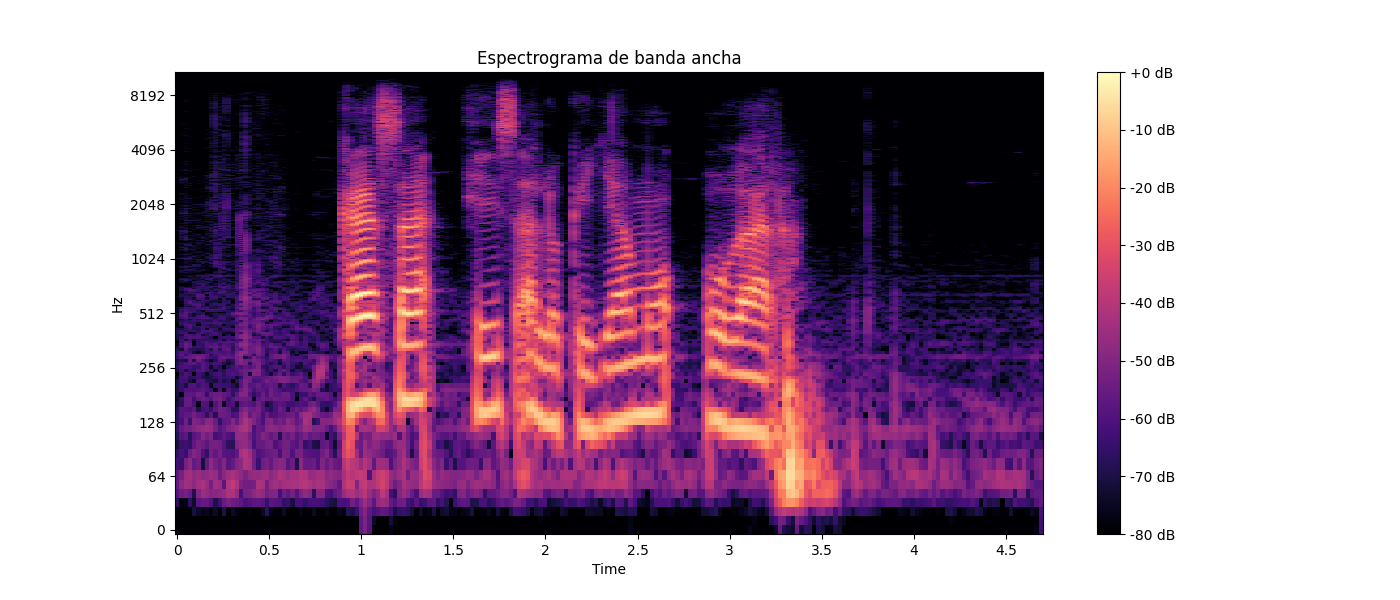
\includegraphics[width=\linewidth]{/audio3/ancha3.png}
        \caption{Espectrograma de banda ancha del audio: Casa es a lo que llamo hogar.}
        \label{fig:espectograma banda ancha audio3}
    \end{figure}
    \item \textbf{Espectrograma de banda estrecha}
    \begin{figure}[h]
        \centering
        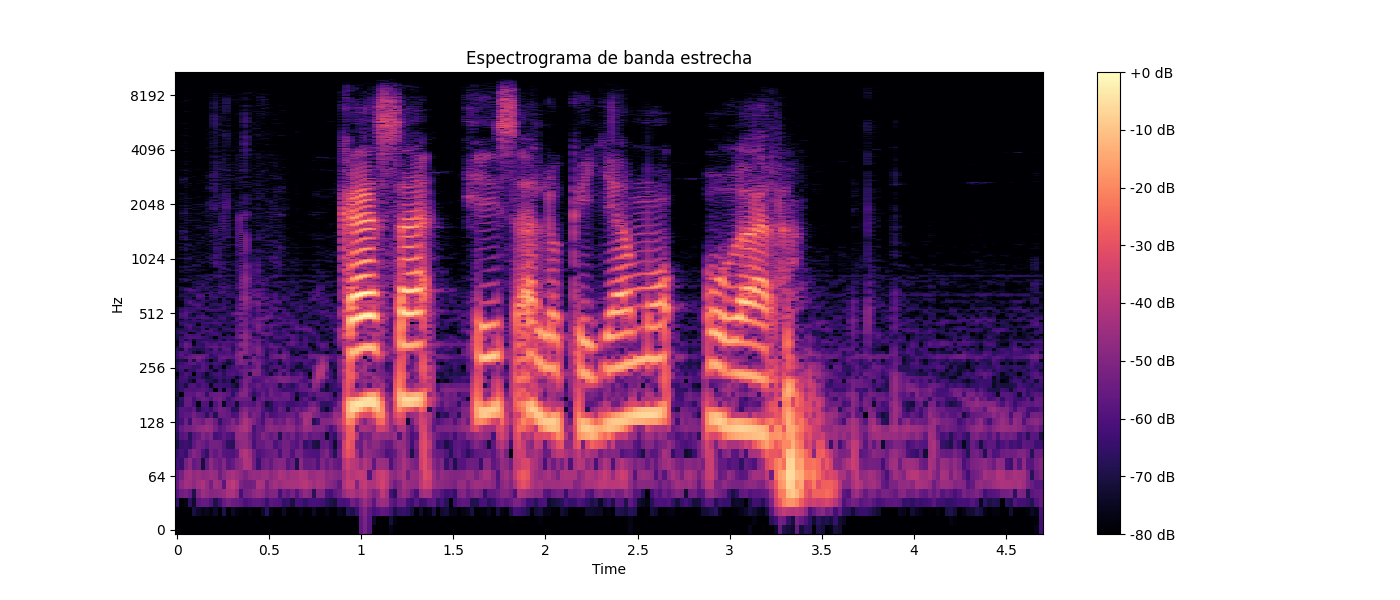
\includegraphics[width=\linewidth]{/audio3/estrecha3.png}
        \caption{Espectrograma de banda estrecha del audio: Casa es a lo que llamo hogar.}
        \label{fig:espectograma banda estrecha audio3}
    \end{figure}
\end{itemize}

\newpage

\subsection{Audio 4 - Los niños juegan en el parque.}
\begin{itemize}
    \item \textbf{Dominio del tiempo con segmentación de 100 ms y etiquetas (S, U, V)}
    \begin{figure}[h]
        \centering
        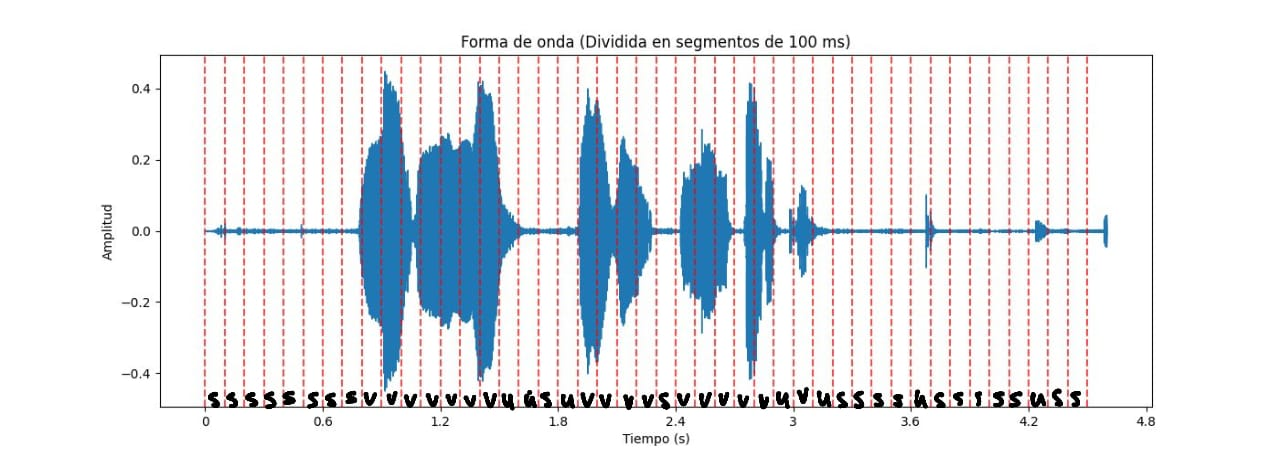
\includegraphics[width=\linewidth]{/audio4/a4.jpeg}
        \caption{Forma de onda del audio: Los niños juegan en el parque.}
        \label{fig:forma_onda_audio4div}
    \end{figure}
    \item \textbf{Forma de onda de la señal de voz completa}
    \begin{figure}[h]
        \centering
        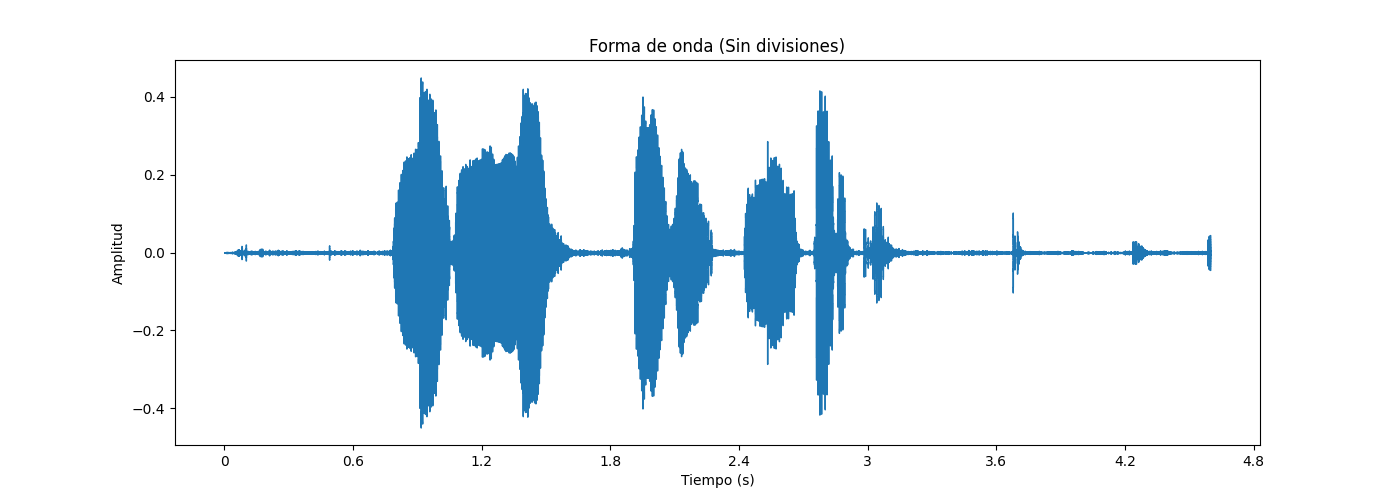
\includegraphics[width=\linewidth]{/audio4/Figure_1a4.png}
        \caption{Forma de onda del audio: Los niños juegan en el parque, con segmentación de 100 ms}
        \label{fig:forma de onda_audio4}
    \end{figure}
    \newpage
    \item \textbf{Espectrograma de banda ancha}
    \begin{figure}[h]
        \centering
        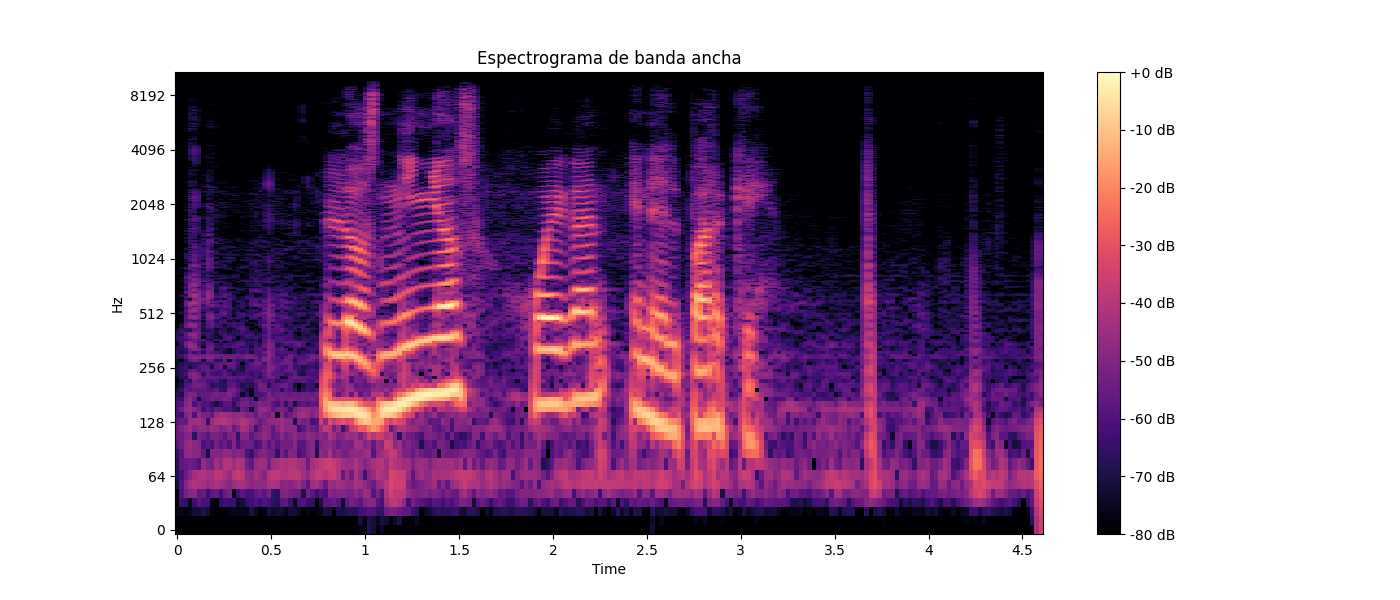
\includegraphics[width=\linewidth]{/audio4/ancha4.png}
        \caption{Espectrograma de banda ancha del audio: Los niños juegan en el parque.}
        \label{fig:espectograma banda ancha audio4}
    \end{figure}
    \item \textbf{Espectrograma de banda estrecha}
    \begin{figure}[h]
        \centering
        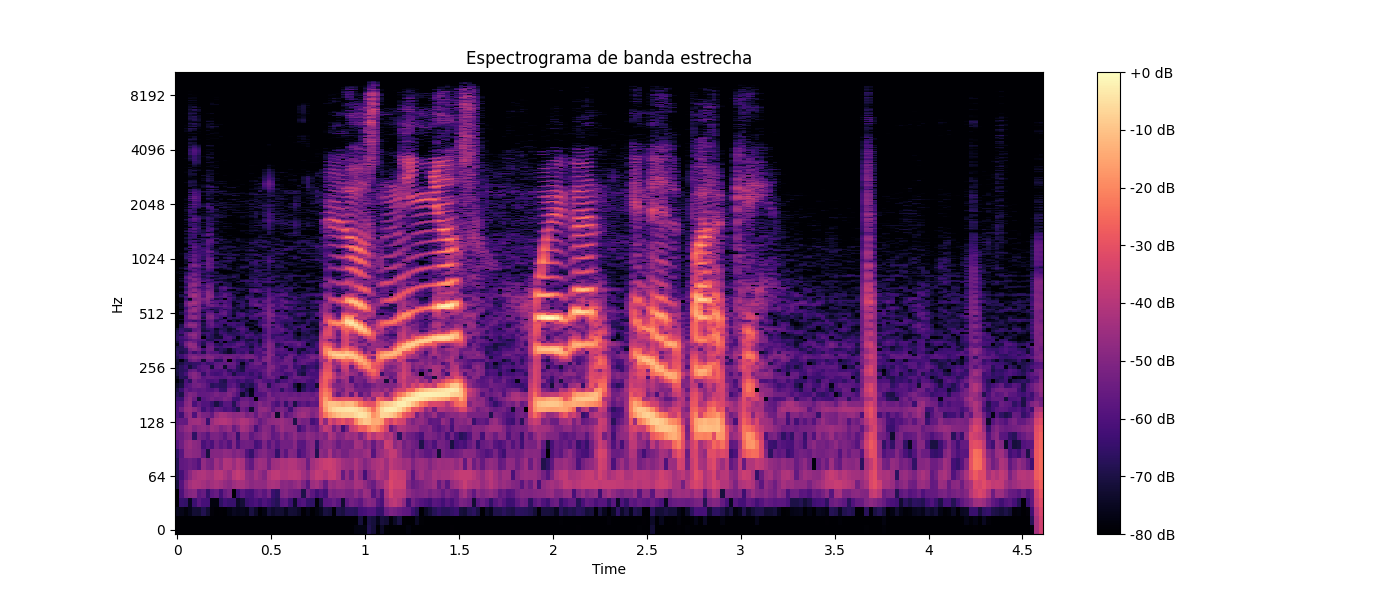
\includegraphics[width=\linewidth]{/audio4/estrecha4.png}
        \caption{Espectrograma de banda estrecha del audio: Los niños juegan en el parque.}
        \label{fig:espectograma banda estrecha audio4}
    \end{figure}
\end{itemize}

\newpage

\subsection{Audio 5 - En la mañana me preparo y salgo a la escuela.}
\begin{itemize}
    \item \textbf{Dominio del tiempo con segmentación de 100 ms y etiquetas (S, U, V)}
    \begin{figure}[h]
        \centering
        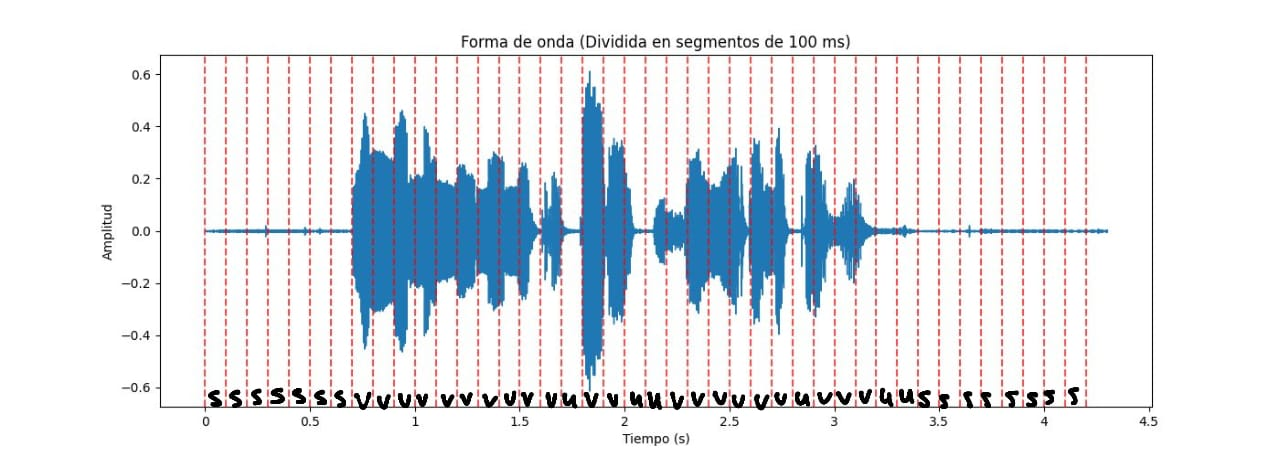
\includegraphics[width=\linewidth]{/audio5/a5.jpeg}
        \caption{Forma de onda del audio: En la mañana me preparo y salgo a la escuela.}
        \label{fig:forma_onda_audio5div}
    \end{figure}
    \item \textbf{Forma de onda de la señal de voz completa}
    \begin{figure}[h]
        \centering
        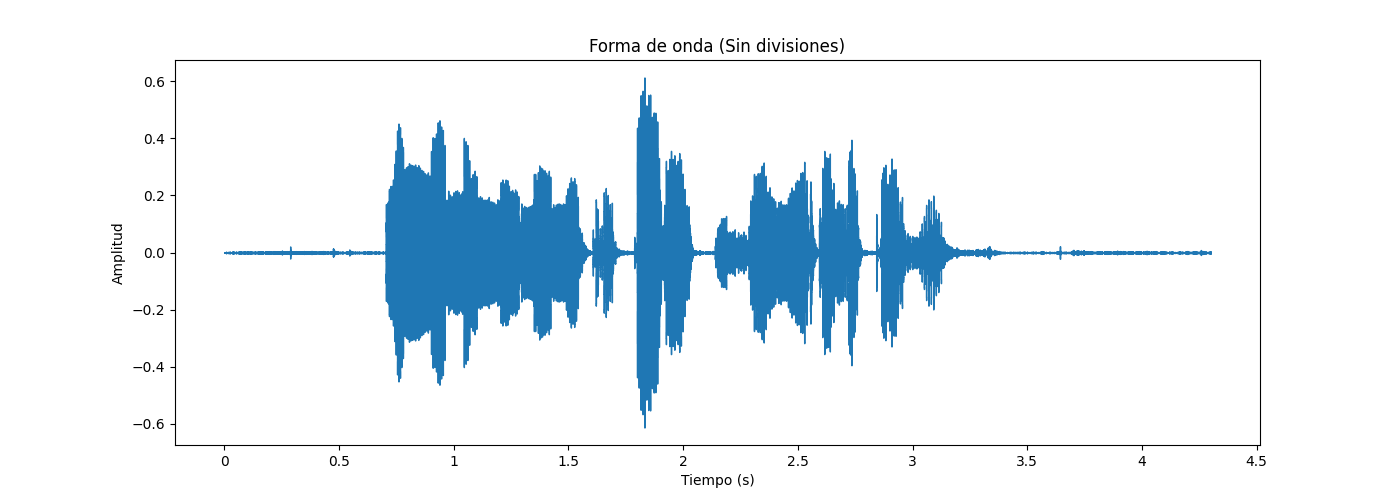
\includegraphics[width=\linewidth]{/audio5/Figure_1a5.png}
        \caption{Forma de onda del audio: En la mañana me preparo y salgo a la escuela, con segmentación de 100 ms}
        \label{fig:forma de onda_audio5}
    \end{figure}
    \newpage
    \item \textbf{Espectrograma de banda ancha}
    \begin{figure}[h]
        \centering
        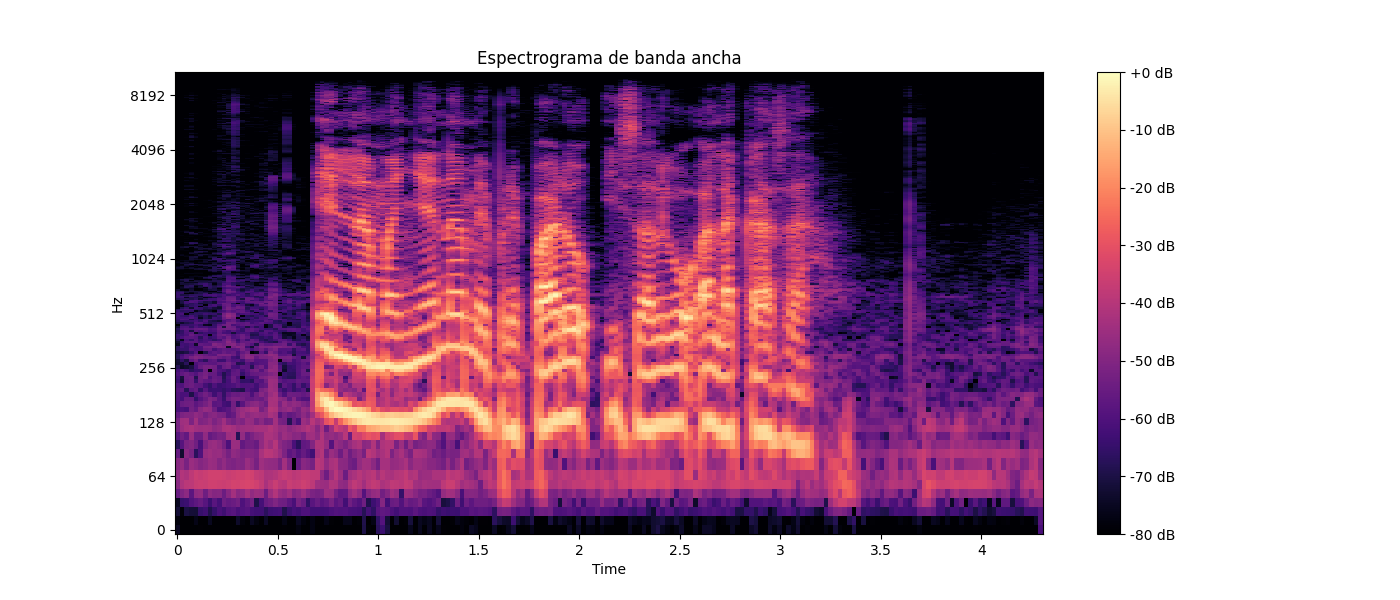
\includegraphics[width=\linewidth]{/audio5/ancha5.png}
        \caption{Espectrograma de banda ancha del audio: En la mañana me preparo y salgo a la escuela.}
        \label{fig:espectograma banda ancha audio5}
    \end{figure}
    \item \textbf{Espectrograma de banda estrecha}
    \begin{figure}[h]
        \centering
        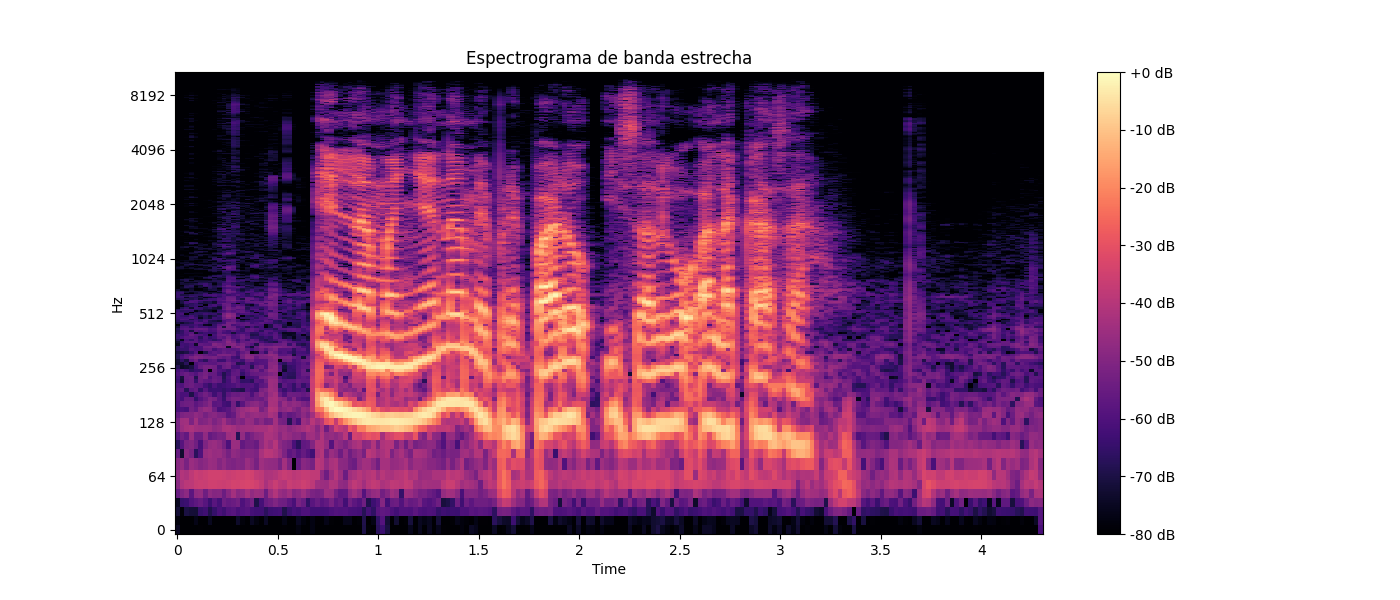
\includegraphics[width=\linewidth]{/audio5/estrecha5.png}
        \caption{Espectrograma de banda estrecha del audio: En la mañana me preparo y salgo a la escuela.}
        \label{fig:espectograma banda estrecha audio5}
    \end{figure}
\end{itemize}

\newpage
\section{Conclusiones}

Los resultados obtenidos para los audios permiten observar cómo varía la energía en diferentes frecuencias a lo largo del tiempo. Esto es útil para identificar patrones de habla, como la aparición de formantes, que son concentraciones de energía en ciertas frecuencias y constituyen características fundamentales de los sonidos del habla.  

Las áreas más oscuras en el espectrograma indican frecuencias con mayor energía, que podrían corresponder a sonidos vocálicos o consonánticos sonoros. Por otro lado, las áreas más claras representan frecuencias con menor energía, asociadas a pausas o sonidos fricativos.  

Asimismo, en la forma de onda se observa la variación de amplitud a lo largo del tiempo, donde los picos corresponden a sonidos más fuertes (como las vocales) y los valles a sonidos más suaves o pausas.  

Si bien las gráficas presentan similitudes para los cinco audios analizados, la comparación entre ellas permite apreciar que los espectrogramas de banda ancha y banda estrecha proporcionan información complementaria. Los espectrogramas de banda ancha resultan útiles para una visión general de la estructura del habla, mientras que los de banda estrecha permiten un análisis más detallado de las frecuencias y los armónicos.  

Por otro lado, las formas de onda son esenciales para comprender la dinámica temporal del habla. Sin embargo, la ausencia de divisiones en los ejes puede dificultar una interpretación precisa de los eventos acústicos.  

Gracias al desarrollo de esta práctica, se logró una mejor comprensión de las representaciones del habla en los dominios del tiempo y la frecuencia. Esto permitirá un análisis más profundo de las señales de voz en futuros proyectos de reconocimiento de voz, ya que el estudio de las formas de onda y los espectrogramas (tanto de banda ancha como de banda estrecha) proporciona una visión detallada de la estructura del habla en términos de amplitud, tiempo y frecuencia.

\newpage
\begin{thebibliography}{00}

    \bibitem{rabiner} L. R. Rabiner and R. W. Schafer, \textit{Theory and Applications of Digital Speech Processing}. Upper Saddle River, NJ, USA: Pearson, 2010.
    
    \bibitem{oppenheim} A. V. Oppenheim and R. W. Schafer, \textit{Discrete-Time Signal Processing}, 3rd ed. Upper Saddle River, NJ, USA: Prentice Hall, 2009.
    
    \bibitem{gold} B. Gold, N. Morgan, and D. Ellis, \textit{Speech and Audio Signal Processing: Processing and Perception of Speech and Music}, 2nd ed. Hoboken, NJ, USA: Wiley, 2011.
    
    \bibitem{stevens} K. N. Stevens, \textit{Acoustic Phonetics}. Cambridge, MA, USA: MIT Press, 1998.
    
    \bibitem{hermansky} H. Hermansky, "Perceptual Linear Predictive (PLP) Analysis of Speech," \textit{Journal of the Acoustical Society of America}, vol. 87, no. 4, pp. 1738-1752, 1990, doi: 10.1121/1.399423.
    
    \end{thebibliography}
    

\end{document}